\begin{frame}
	\frametitle{Classificazione dei dati di conformance}
	\begin{figure}
	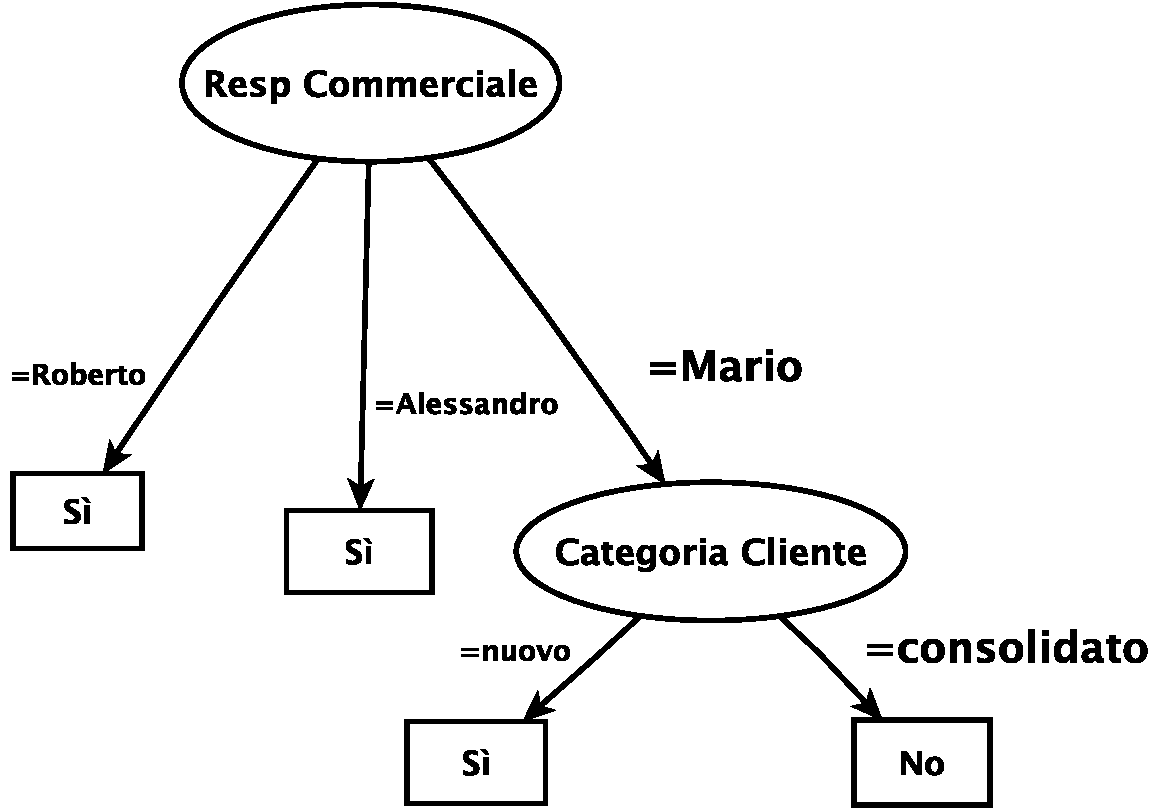
\includegraphics[scale=0.3]{./fig/decisiontree}
	\end{figure}
	\begin{block}{}
	\begin{itemize}
	\item Alcune istanze non sono conformi al modello: la comunicazione al cliente avviene prima della terminazione delle valutazioni.
	\item Gli ordini gestiti da Mario e fatti da clienti consolidati non rispettano la procedura.
	\end{itemize}
	\end{block}
	\end{frame}
	
	\begin{frame}
	\frametitle{Possibili misure correttive}
	\begin{block}{A livello di processo}
	Riorganizzazione del processo aziendale: giudicare ragionevole saltare le fasi di valutazione per i clienti consolidati.
	\end{block}
	\begin{figure}
	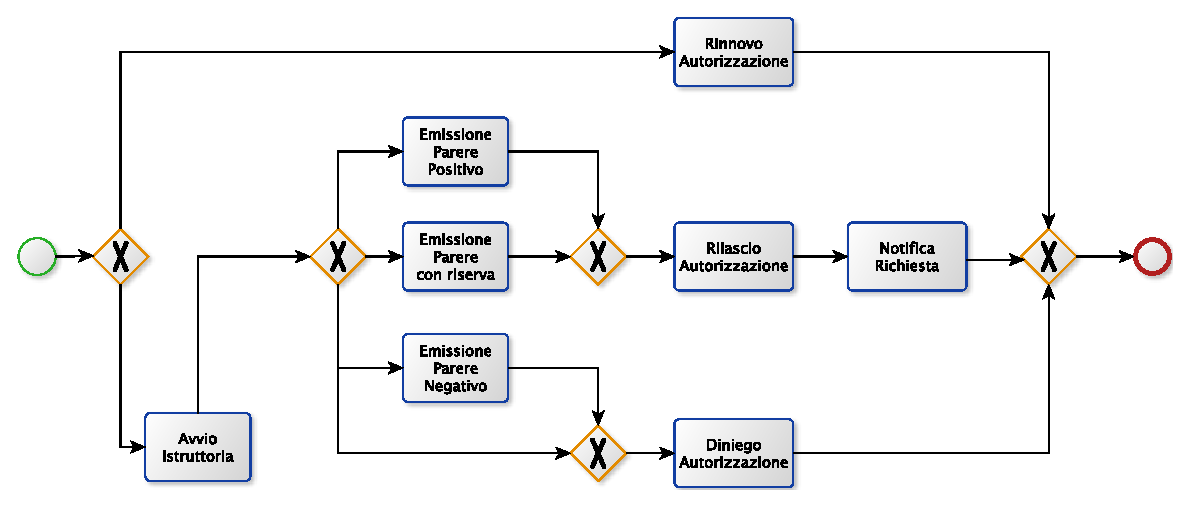
\includegraphics[scale=0.4]{./fig/BPMN}
	\end{figure}
	\begin{block}{Predizione}
	Uso del classificatore in senso predittivo: prevedere i casi di non conformità con segnalazione al personale per evitare errori noti.  
	\end{block}
	\end{frame}
	